\newpage
\appendix
\section{Appendix}\label{app}
\subsection{Choice of Equilibria}\label{sec:equi}
When dropping the assumption that a player needs to be as fast as possible at every intermediate node and instead only needs to arrive as early as possible at the destination, strange behavior patterns can arise that do not necessarily mirror the behavior of road traffic participants in reality. In particular, there might be instances where players with a higher index can arrive at intermediate nodes strictly earlier than players with a lower index and therefore overtake a player with higher priority for some time. Only due to the tie-breaking rules, they will later be overtaken again.  
Consider the following graph, visualized in Figure \ref{fig:overtakingInNE}, with the strategy profile
$P_{(1)}=(e_1^1,e_1^2,e_1^3), P_{(2)}=(e_2^1,e_2^2,e_1^3)$, $P_{(3)}=(e_3^1,e_1^2,e_1^3)$, $P_{(4)}=(e_1^1,e_2^2,e_1^3)$, $P_{(5)}=(e_2^1,e_1^2,e_1^3)$, $P_{(6)}=(e_3^1,e_2^2,e_1^3)$, $P_{(7)}=(e_1^1,e_1^2,e_1^3)$, \mbox{$P_{(8)}=(\mathbf{e_4^1},e_2^2,e_1^3)$}, $P_{(9)}=(e_2^1,e_2^2,e_1^3)$.
Clearly, due to all players arriving at $t$ in order of their index one at a time beginning at time $3$ all players arrive as early as possible at the destination. Note that player 8 takes a detour by taking the longer edge $e_4^1$ and is strictly later at node $v_1$ than player 9, while arriving at $d$ strictly before player $8$. Hence this state is not an UFR equilibrium but all players arrive as early as possible at the destination.
\begin{figure}[h]
    \centering
    \tikzstyle{vertex}=[circle,fill=black!25,minimum size=20pt,inner sep=0pt]
\tikzstyle{smallvertex}=[circle,fill=black,minimum size=6pt,inner sep=0pt]
\tikzstyle{edge} = [draw,thin,->]
\tikzstyle{weight} = [font=\small]
\tikzstyle{selected edge} = [draw,line width=3pt,-,red!50]
\tikzstyle{big edge} = [draw,line width=2pt,->,black]
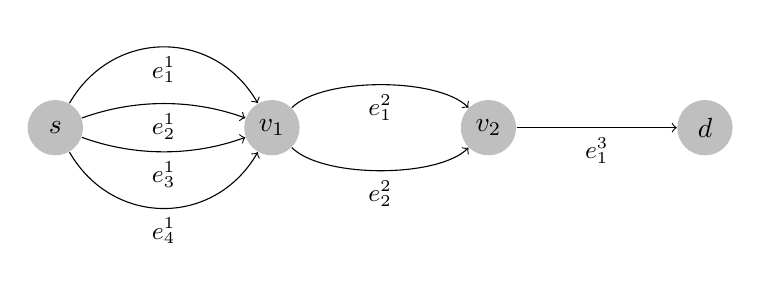
\begin{tikzpicture}[scale=0.55,auto,swap]
    \node[vertex](s1) at (0,0){$s$};
    \node[vertex](s2) at (5,0){$v_1$};
    \node[vertex](s3) at (10,0){$v_2$};
    \node[vertex](s4) at (15,0){$d$};

    \draw [edge] (s1) to[out=60,in=120, distance=2cm ] node[weight,below,black]{$e_1^1$} (s2);
    \draw [edge] (s1) to[out=20,in=160, distance=1.3cm ] node[weight,below,black]{$e_2^1$} (s2);
    \draw [edge] (s1) to[out=-20,in=200, distance=1.3cm ] node[weight,below,black]{$e_3^1$} (s2);
    \draw [edge] (s1) to[out=-60,in=240, distance=2cm ] node[weight,below,black]{$e_4^1$} (s2);
    
    \draw [edge] (s2) to[out=45,in=135, distance=1cm ] node[weight,below,black]{$e_1^2$} (s3);
    \draw [edge] (s2) to[out=-45,in=-135, distance=1cm ] node[weight,below,black]{$e_2^2$} (s3);

    \draw [edge] (s3) to[out=0,in=180, distance=1cm ] node[weight,below,black]{$e_1^3$} (s4);
 \end{tikzpicture}
    \caption{The transit time of edge $e_4^1$ is $4$. All other edges have a transit time of $1$. Network, in which there is a state for $9$ players, where player 9 is strictly earlier at node $v_1$ than player 8, while simultaneously all players arrive as early as possible at the destination $d$.}
    \label{fig:overtakingInNE}
\end{figure}
% \clearpage
\subsection{Omitted Proof of Section \ref{sec:understandingopt}}\label{app:understandingopt}

\satzOptStructure*
\noindent
\begin{proof}
    Ford and Fulkerson~\cite{ford1958constructing} showed that a packet routing maximizing the number of packets arriving at $d$ until $T$ in linear multigraphs with edge capacity equal to one can be computed by deleting shortest paths as long as the distance $dist(s,d)$ is smaller than $T$.
        \begin{enumerate}
        \item Initialize $x_P=0$ for all $P\in \mathcal{P}$.
        \item WHILE $dist(s,d)\leq T$:\\
        $\qquad$ Compute a shortest $s-d$ path $P$ in $G$, delete $P$ from $G$ and set $x_P = 1$.
        \item Return a temporally repeated flow $\tilde{S}$ for $(x_P)_{P\in \mathcal{P}}.$
        \end{enumerate}
    %
    The temporally repeated flow $\tilde{S}$ is defined as follows. For all paths $P$ with $x_P = 1$ it sends packets into $P$ at time steps $\{0, 1, \dots, T-\tau(P)\}$. It is worth noting that for arbitrary graphs one needs to base the calculations above on the residual graphs. Here, we could simplify the algorithm as linear multigraphs are series-parallel and a shortest $s-d$ path would never use any backward edge in the residual graph.
    
    It is immediate to see that when instead sending $T-\tau(P)$ packets into $P$ at time $0$ and stopping afterwards, all packets immediately enter the queue of the first link. We obtain a state of the packet routing game where no packet waits outside of the first layer. 
    
    To finish the proof, fix an arbitrary optimal state $S^*$ for the packet routing game with $n$ players with latest arrival time $C(S^*)$. By~\cite{ford1958constructing} there is a temporally repeated flow $\tilde{S}$ for time horizon $C(S^*)$ sending $n'\geq n$ packets to $d$ up to time $C(S^*)$. If $n'> n$, we have $n' = j + n$ for some $1\leq j\leq k-1$, since otherwise $\Tilde{S}^*$ would not be optimal. To send the correct amount of packets, we delete the last packet from each of the paths $P^k,P^{k-1},\ldots, P^{k-j+1}$. Since $\tilde{S}$ is feasible, the obtained flow is also feasible. We have constructed an optimal state that fulfills all claimed properties.
    %
    %there is a flow over time that sends flow of mass $n$ from $s$ to $d$ until time $C(\Tilde{S}^*)+1$. In particular, the earliest arrival flow $f$ from above does this. As $G(\Gamma)$ is a linear multigraph and thus in particular a serial-parallel graph, only forward edges will be used in the algorithm. Hence, the resulting flow of the algorithm is a temporally repeated flow, i.e., it sends over edge-disjoint paths $P^1,\ldots, P^k$ a flow with static flow value of 1 in the time interval $[0, C(S)-\tau(P^j))$ for any $j\leq k$. Since all $\tau_e$ and $C(\Tilde{S}^*)$ are integers, the flow $f$ is piecewise constant with a jump at an integer value at $C(\Tilde{S}^*)-\tau(P^j)-1$ on the from $s$ outgoing edge $e$ with $e\in P^j$.
    %We construct an optimum state $S^*$ by sending a packet over an edge $e$ at time $t$ with a flow value of 1 in the interval $[t,t+1)$. Since $f$ is temporally repeated, it fulfills the strong flow conservation and, hence, no packet is ever waiting at any intermediate node.  Since the last flow particle in $f$ arrives at time $C(\Tilde{S}^*)+1$ at $d$, the last packet in $S^*$ arrives at $d$ at $C(\Tilde{S}^*)$, i.e., $C(S^*) = C(\Tilde{S}^*)$. 
\end{proof}
% \clearpage

\subsection{A Model Extension to Arbitrary Edge Capacities}\label{sec:edgcap}
We can generalize the model by allowing edges $e$ to have capacities $\nu_e\in \N_{>0}$ which may differ from one. In contrast to the model presented in the Section \ref{sec:prelim}, in the network loading process at any point in time, $\nu_e$ players are now allowed to leave the queue $q_e$. In this section, we will argue, with the help of a reduction, that the $\PoA$ and the $\PoS$ are still bounded as in the base model.

Given a game $\Gamma$ with edge capacities that may differ from one, we can construct a game $\Gamma'$ by replacing every edge $e=(v,w)$ with transit time $\tau(e)$ and capacity $\nu_e$ by $\nu_e$ many edges $e^1, \ldots,e^{\nu_e}=(v,w)$ each with transit time $\tau(e)$ and unit capacity.
For an arbitrary equilibrium $S$ of $\Gamma$, we can construct a strategy profile $S'$ of $\Gamma'$ as follows: for each player $i$, we replace in the player's strategy every edge $e\in P_{(i)}$ by $e^j$, where $j=((q_e(i)-1 )\mod \nu_e)+1$. In this context, $q_e(i)$ denotes the queuing position of player $i$ on edge $e$ when she uses this edge. As a result of this construction, the arrival times at every node and, consequently, the completion times are identical, that is, $C^{\Gamma}(S)=C^{\Gamma'}(S')$. Furthermore, $S'$ is an equilibrium of $\Gamma'$. If this were not the case, there would exist a player who could strictly improve her completion time by changing her strategy. By changing her strategy in $S$ to the corresponding edges she achieves a better completion time in $\Gamma$. This contradicts the fact that $S$ is an equilibrium. Therefore, we have 
$$\sup_{S\in \Nash^{\Gamma}} C^{\Gamma}(S) \leq \sup_{S'\in \Nash^{\Gamma'}} C^{\Gamma'}(S').$$
Let $S^*$ be an optimal state of $\Gamma$ and $(S')^*$ be the strategy profile of $\Gamma'$ that arises from the transformation of $S^*$ as described above. The optimal completion time in $\Gamma'$ is at most as big as $C^{\Gamma'}((S')^*)=C^{\Gamma}(S^*)$. 
In total, we obtain a game $\Gamma'$ with unit capacities for every game $\Gamma$ with $\PoA(\Gamma)\leq \PoA(\Gamma')$. Hence, we can apply Theorem \ref{satz_PoA2} to conclude that
\begin{align*}
    \PoS(\mathcal{H}) \leq \PoA(\mathcal{H}) = \sup\limits_{\Gamma: G(\Gamma) \in \mathcal{H}} \PoA(\Gamma) \leq \sup\limits_{\Gamma': G(\Gamma') \in \mathcal{H}, \nu_e = 1 \forall e} \PoA(\Gamma') \leq 2.
\end{align*}
In conjunction with Theorem \ref{satz_PoAgeqee1}, this leads to the conclusion that for the extended model with edge capacities, it holds that $$\frac{e}{e-1}\leq PoS(\mathcal{G}) \leq \PoA(\mathcal{G})\leq 2.$$ 

% \clearpage
\subsection{Omitted Proofs of Section \ref{sec:poa}}\label{app:sec4}
\lemmaAli*
\begin{proof}
As defined in the network loading, we refer to an edge as \emph{used (at time $t$)} when a player leaves the queue of this edge at time $t$.
If, at any time $t$, there is a used edge $e^1_j$ that has a strictly higher %latency
workload than another used edge $e^1_i$ with $i<j$, then the player with the largest index queuing on edge $e^1_j$ could have chosen edge $e^1_i$ without worsening her latency since the queue lengths on all used edges decrease at the same rate. This contradicts the assumption that the player behaves according to \badNash.

Conversely, suppose at some time $t$, there is a used edge $e^1_j$ and another used edge $e^1_i$ with $i<j$ and $l_{e^1_j}(\badNash,t)+1<l_{e^1_i}(\badNash,t)$.
Then the player with the largest index to queue on edge $e_i$ could have chosen edge $e_j$ instead. This contradicts the assumption that we are in an equilibrium.
Together this yields $l_{e^1_j}(\badNash,t) \leq l_{e^1_i}(\badNash,t) \leq l_{e^1_j}(\badNash,t)+1$.
\end{proof}

\lemmaOneLayerNew*
\begin{proof}
In the network loading at time $t$, we first add every player entering an edge to the queue and then remove the first player from each queue. For any $S \in \Nash$, we denote the sum of queue lengths in the network at time $t$ after the removal by $Q(S,t)$. When comparing $Q(S,t)$ to $Q(S,t-1)$ observe that we can obtain $Q(S,t)$ from $Q(S,t-1)$ as follows. We denote the number of players starting at time $t$ with $Q^+(S,t)$. For every player with starting time $t$, we increase the sum of queue lengths by one. Afterwards, the total queue length decreases by the number of used edges at time $t$, i.e., edges with a non-empty queue, denoted by $Q^-(S,t)$. Thus, we have $Q(S,t)= Q(S,t-1)+Q^+(S,t)-Q^-(S,t)$.
\paragraph{Claim:} $Q(\badNash,t) \geq Q(S,t)$ for all $S\in \Nash$ and for all $t\in \N_{>0}$.

\noindent \textit{Proof of claim.}
Suppose there exists a state $S\in \Nash$ and a time $t\in \N_{>0}$ such that $Q(\badNash,t) < Q(S,t)$. 
Consider the earliest point in time $t'$ at which this happens. Thus, we know that $Q(\badNash,t'-1) \geq Q(S,t'-1)$ and $Q^+(S,t')= Q^+(\badNash,t')$.
We conclude that $Q^-(\badNash,t') > Q^-(S,t')$, i.e., $\badNash$ uses strictly more edges at $t'$ than $S$ does.
We call an edge $e$ \emph{new} (at time $t'$) if the queue $q_e$ at time $t$ is empty, i.e., the first player entering the edge experiences no queuing time on this edge. Conversely, we call an edge \emph{old} (at time $t$) if it is not new at time $t$. Furthermore, the first player on a new edge does not contribute to $Q(S,t')$, since this player is counted in $Q^+(S,t')$ as well as in $Q^-(S,t')$. 

Hence, $\badNash$ uses more new edges than $S$. Let $e'$ be a new edge exclusively used by $\badNash$ at $t'$. By Lemma \ref{lemma_ali}, \badNash\ also uses all edges with transit time smaller than $\tau(e')$ at time $t'$. Furthermore, $S$ cannot use an edge with a larger transit time than $\tau(e')$ without contradicting the equilibrium property. Since $S$ has more players in queues, there has to be an edge $e''$ which has more players in its queue under $S$ than under $\badNash$ at time $t'$.


Due to Lemma \ref{lemma_ali}, we know that in $\badNash$ new edges are only used if each edge with a smaller index has a strictly higher %latency
workload. Additionally, in $S$, the queue on $e''$ is even longer than in \badNash. Summarizing, $l_{e''}(S,t')\ge l_{e'}(S,t')+2 = \tau(e')+2$.
Consequently, the last player on $e''$ in $S$, which experiences a latency of at least $\tau(e')+1$, can improve her latency by changing her strategy to $e'$. This contradicts the assumption that $S$ is an equilibrium.\qed

\medskip
%
\noindent Furthermore, we observe that the completion time of any player $i$ starting at $t+1$ is uniquely defined given the total queue length $Q(S,t)$ at time $t$ for any $S\in \Nash$, since the $Q(S,t)$-many players in queues level out the latencies on the shortest edges. This suffices to determine the latencies of the subsequent players. Additionally, the completion time of player $i$ is monotonically increasing in $Q(S,t)$. This yields $C_i(\badNash)\geq C_i(S)$ for all $S \in \Nash$ and all $i\in N$.
\end{proof}


\lemmaMnKStartpattern*
\noindent
\begin{proof}
It is sufficient to show that the statement holds for starting patterns $a$ and $b$ which differ in only one entry by one. Then, a general $a$ can be transformed into $b$ by step-wise transformations. 

Let $a$ and $b$ be such starting patterns and $\ell$ be the index at which the patterns differ, that is $a(\ell)+1=b(\ell)$. Note that player $\ell$ is the player with the largest index of her generation in $a$ and the player with the smallest index of her generation in $b$. Obviously, $C_{\ell}(\badNash^a)\le C_{\ell}(\badNash^b)$, since all players up to player $\ell-1$ choose the same strategy under the greedy queue policy and $\ell$ could use the same edge under both starting patterns. Note that $C_\ell(\badNash^a) = C_\ell(\badNash^b)$ if and only if $\ell$ has to wait under starting pattern $a$, i.e., $\ell$ uses an old edge with a non-empty queue.

\paragraph{Claim:} If $C_\ell(\badNash^a) = C_\ell(\badNash^b)$, we have $\badNash^a = \badNash^b$.

\noindent \textit{Proof of claim.} Both $\badNash^a$ and $\badNash^b$ arise from the greedy queue policy $\phi$, i.e., is the same for all players up to $\ell-1$ as the graph and the starting times are the same up to player $\ell-1$. Given this setup, $\phi$ allocates the edge with the smallest workload to $\ell$ where ties are broken in favor of longer queues. As observed above, $\ell$ is allocated to some edge $\badNash^a_{(\ell)}$ with queue under $\badNash^a$. The arrival time of $\ell$ on the same edge under $b$ is obviously the same, thus, this is still the fastest edge with the longest queue under $b$. Hence, $\badNash^a_{(\ell)} = \badNash^b_{(\ell)}$ with the same arrival time of $\ell$, i.e., nothing changes for all subsequent players and $\badNash^a = \badNash^b$.\qed

\medskip
%
\noindent This finishes the proof for the case $C_\ell(\badNash^a) = C_\ell(\badNash^b)$.
On the other hand, if player $\ell$ arrives earlier because she starts one time unit earlier at $s$, then she does not queue, i.e., she uses an unused edge. As this edge is also unused when $\ell$ starts one time step later, we observe $C_\ell(\badNash^a) = C_\ell(\badNash^b) -1$. It remains to show that $C_i(\badNash^a) \leq C_i(\badNash^b)$ for all $i > \ell$. 

We add an additional dummy player to the player set with an index between $\ell$ and $\ell+1$, where the starting time of the dummy is the same as of $\ell+1$. As we consider the greedy queue policy and $\ell$ did not queue, the dummy uses the edge of player $\ell$ under $b$. Since the subsequent players now face the exact same situation in our new game with starting pattern $a$ and the additional dummy as in $b$, $C_i(\badNash^a) = C_i(\badNash^b)$ for all $i\geq\ell +1$.

Now, we will carefully modify the priority of the dummy and swap it with the subsequent players generation by generation. While doing so, we observe that the arrival times $C_i(\badNash^a)$ do not increase. For the generation of player $\ell +1$, we sequentially swap the priorities and strategies of the dummy with its subsequent player. This swap only changes the strategies of the dummy and the subsequent player and may decrease the arrival time of the subsequent player. As this swap does not change queue lengths, all other players still behave according to the greedy queue policy. Thus, the new state is an equilibrium according to greedy queue. We can continue this procedure until the dummy player is the player with the largest index of its generation. Note that the swaps might have increased the dummy player's arrival time. 

If the dummy has the largest index in its generation, we have two cases. 

\paragraph{Case 1:} If the dummy player is in a queue, we increment its generation by one, i.e., it is now the player with the smallest index of the next generation and starts one time unit later. Now, the same argument as in the claim holds for the dummy and she chooses the same edge under the policy greedy queue. We continue and iterate the swapping until the dummy is again the player with the largest index of the generation.
\paragraph{Case 2:} If the dummy player uses an edge without queue or is the player with the largest index, we delete the dummy player. In the first subcase, deleting the dummy does not change the queues for the player after the dummy, as this player could even take the dummy's edge without observing any queue. In the second subcase, the dummy was the player with the largest index, and deleting the dummy trivially does not change $C(\badNash^a)$.\\

\noindent Finally, we have started with $C_i(\badNash^a) = C_i(\badNash^b)$ for all $i>\ell$ and we have never increased $C_i(\badNash^a)$ during the dummy swaps. Thus, we have $C_i(\badNash^a)\leq C_i(\badNash^b)$ for all $i\in N$. 
\end{proof}

\lemmaAddingEdges*
\noindent
\begin{proof}
It is sufficient to show that the property holds for $|E_2\backslash E_1|=1$. Let $e=(v_j,v_{j+1})$ be the edge where the two graphs differ. Up to node $v_j$ the arrival patterns $a_{v_j}(\badNash_{G_1})$ and $a_{v_j}(\badNash_{G_2})$ trivially coincide.
Suppose that there is a player $i$ such that $a^i_{v_{j+1}}(\badNash_{G_2}) > a^i_{v_{j+1}}(\badNash_{G_1})$ and $a^{i'}_{v_{j+1}}(\badNash_{G_2}) \leq a^{i'}_{v_{j+1}}(\badNash_{G_1})$ for all $i'<i$. In particular, there are at most $|\{e\in E_1^{j+1}: \tau(e) \leq a^i_{v_{j+1}}(\badNash_{G_1}) - a^i_{v_{j}}(\badNash_{G_1})\}| -1$ players with index less than $i$ that arrive at $v_{j+1}$ at time $a^i_{v_{j+1}}(\badNash_{G_1})$. Here $E_1^{j+1}$ denotes the edges in $E_1$ that are in the $(j+1)$-th layer of $G_1$. Since $i$ arrives at $v_{j+1}$ strictly later in $G_2$ than in $G_1$, among all edges of $\{e\in E_1^{j+1}: \tau(e) \leq a^i_{v_{j+1}}(\badNash_{G_1}) - a^i_{v_{j}}(\badNash_{G_1})\}$ players arrive at $v_{j+1}$ at time $a^i_{v_{j+1}}(\badNash_{G_1})$ in $\badNash_{G_2}$. Note, that is one more player. By Lemma \ref{lemma_order} the additional player $i'$ has $i'<i$, since no overtaking is possible at any intermediate node in any equilibrium. But then we have $a^{i'}_{v_{j+1}}(\badNash_{G_2}) > a^{i'}_{v_{j+1}}(\badNash_{G_1})$, which contradicts that player $i$ was the player with the smallest index that was delayed. Therefore, $a^i_{v_{j+1}}(\badNash_{G_1}) \geq a^i_{v_{j+1}}(\badNash_{G_2})$ holds for all $i\in N$.
In the later layers, the graphs are indistinguishable. Therefore, by iterating node by node to the destination node $d$, we obtain the statement by applying Lemma $\ref{lemma_mnK_startpattern}$ at each step.
\end{proof}

%\clearpage
%\subsection{Omitted Proof of Section \ref{sec:posBadInst}}\label{app:sec5}
%\satzPoAgeqee*
%\noindent
%\begin{proof}[Remaining Part]
%\end{proof}

% \clearpage
\subsection{Basic Notations for Flows over Time and Omitted Proof of Section \ref{sec:FlowOverTime}}\label{app:FlowOverTime}

Flows over time can essentially be seen as the continuous variant of packet routings. For a comprehensive introduction to the topic, we refer to the survey article of Skutella~\cite{Skutella2009survey}. We will follow its lines and recall the most basic definitions here. For a given graph $G$ with transit times $\tau(e)$ for the edges $e \in E$, a designated source $s$, destination $d$ and a fixed time horizon $T$, a flow over time is formally defined as follows.

\begin{definition}
A flow over time $f$ with time horizon $T$ consists of a Lebesgue-
integrable function $f_e : [0, T) \rightarrow \mathbb{R}_{\geq 0}$ for each arc $e \in E$. For all $\theta \geq T - \tau(e)$ it must hold that $fe(\theta) = 0$ for all $e \in E$.
\end{definition}

\begin{definition}
    A flow over time $f$ is called feasible if the following properties hold.
    \begin{enumerate}
    \item The flow over time $f$ fulfills the capacity constraints if $f_e(\theta) \leq \nu_e$ for
each $e \in E$ and almost all $\theta \in [0, T )$.
    \item The flow over time $f$ fulfills the weak flow conservation constraints if the amount of flow that has left a node $v \in V\setminus \{s,d\}$ is always upper bounded by the amount of flow that has entered the same node for all $\theta \in [0,T)$. Formally,
    \[\sum_{e \in \delta^-(v)}\int_0^{\theta - \tau(e)}f_e(\xi)\,d\xi \geq \sum_{e \in \delta^+(v)}\int_0^{\theta}f_e(\xi)\,d\xi\;,\]
    where $\delta^-(v)$ and $\delta^+(v)$ denote the set incoming and outgoing of edges of $v$, respectively.
    \end{enumerate}
\end{definition}
\noindent We say that the amount of flow that has entered $d$ up to time $T$ is the value of the flow $f$. Formally, $|f| = \sum_{e \in \delta^-(d)}\int_0^{T - \tau(e)}f_e(\xi)\,d\xi$. If the weak flow conservation constraint is fulfilled with equality for all $\theta$ and all $v \in V\setminus\{s,d\}$, we say the flow fulfills strong flow conservation. A very special and important class of flows over time are temporally repeated flows. For a feasible static flow $x$ on the same graph, let $(x_P)_{P\in \mathcal{P}}$ be a path decomposition of $x$. The temporally repeated flow $f$ sends flow at rate $x_P$ into $P$ from $s$ during the time interval $[0,T-\tau(P))$. Here, $\tau(P)\coloneqq \sum_{e \in P}{\tau(e)}$ denotes the length of the path $P$. Formally,

\begin{definition}
For a static flow $x$ with flow decomposition $(x_P)_{P \in \mathcal{P}}$ the corresponding temporally repeated flow $f$ with time horizon $T$ is defined by
\[f_e(\theta) \coloneqq \sum_{P \in P_e(\theta)} x_p \qquad \text{for }e=(v,w) \in E, \theta \in [0,T),\]
where $$P_e(\theta) \coloneqq \left\{P \in \mathcal{P} : e \in P \wedge \tau(P_{s,v}) \leq \theta \wedge \tau(P_{v,t}) < T-\theta \right\}.$$ Here, $\tau(P_{u,v})$ denotes the length of $P$ from $u$ to $v$.
\end{definition}
\noindent It is easy to see that temporally repeated flows are feasible and fulfill strong flow conservation, see~\cite{Skutella2009survey}.

A dynamic Nash equilibrium, also called a Nash flow over time, is a special flow over time. It is assumed, that flow appears with a fixed inflow rate at the source node. Similar to the discrete model, the flow is interpreted as an infinite amount of flow particles each deciding at the time of appearance at the source node on a shortest $s-d$ path in a dynamic Nash equilibrium. More formally, for any point in time $\theta \in \mathbb{R}_{\geq 0}$ a positive flow entering an edge $e \in E$ implies that $e$ lies on a currently fastest path to $d$. The makespan-$\PoA$ and makespan-$\PoS$ are defined analogously to the packet routing game, i.e., we compare the latest arrival time of any particle in a Nash flow over time to the arrival time in an optimal flow. Note that for Nash flows over time we even have $\PoA(\mathcal{G})=\PoS(\mathcal{G})$ since the arrival times of dynamic Nash flows over time are unique as recently shown by Olver et al.~\cite{DBLP:conf/focs/OlverSK21}.
% For the remainder of the section, we only consider the makespan-$\PoA$.
For a formal introduction to Nash flows over time, we refer to the PhD theses of Laura Vargas Koch~\cite{PhDLaura} and Leon Sering~\cite{PhDLeon}.


\propositionFlowOverTimeLowerBound*
\begin{proof}
We adapt the graphs used in the proof of Theorem \ref{satz_PoAgeqee1} by omitting the first layer and introducing a constant inflow of $k$ at $s$. We interpret the $n$ players as a flow mass of $n$ similar to the interpretation used by Fleischer and Tardos~\cite{DBLP:journals/orl/FleischerT98}. It remains to argue that the obtained flow over time is indeed feasible and a Nash flow.

Starting with an arbitrary equilibrium $S_i\in \Nash$ of $\Gamma_i$, we construct the Nash flow over time as follows. We set $f_e(\theta)=1$ in the interval \mbox{$[t-1,t)$} whenever a packet leaves the queue $q_e$ of an edge $e=(u,v)$ at time $t$. The constructed flow over time is feasible as we only forward packets if they have already arrived at the corresponding node, thus we immediately respect weak flow conservation in the flow over time. Additionally, as there is at most one packet leaving any queue at a given time, thus we respect the capacity constraints. Regarding the Nash condition observe that at each discrete point in time, a standard edge of some layer is used if and only if all other standard edges are also used as the total number of packets is divisible by any \mbox{$j\in \{1,\ldots, k\}$}. Thus, the standard edges of a layer are used equally, and it is immediate that no standard edge has a strictly lower workload than some other standard edge of the same layer. Additionally, the special edges have strictly larger workloads and are never part of the shortest path network. Since the first omitted layer consists exclusively of standard edges with a transit time of one, we respect the inflow into the network. The completion time of the dynamic Nash equilibrium is by definition $C(S_i)$.

It remains to bound the completion time of an optimal flow over time in this instances. In series-parallel graphs, there is a temporally repeated flow over time that is also an earliest arrival flow, i.e., a flow that maximizes the flow that arrived at $d$ at any point in time, see~\cite{Skutella2009survey}. In particular, this flow is optimal for minimizing the completion time. By Proposition~\ref{thm:opt} the completion time of this earliest arrival flow and the optimal packet routing coincide up to one and we conclude in the limit $\PoA(\mathcal{G})\geq \frac{e}{e-1}$.
\end{proof}
